\documentclass[tikz]{standalone}
\usepackage{pgfplots}
\pgfplotsset{compat=1.18}

\begin{document}

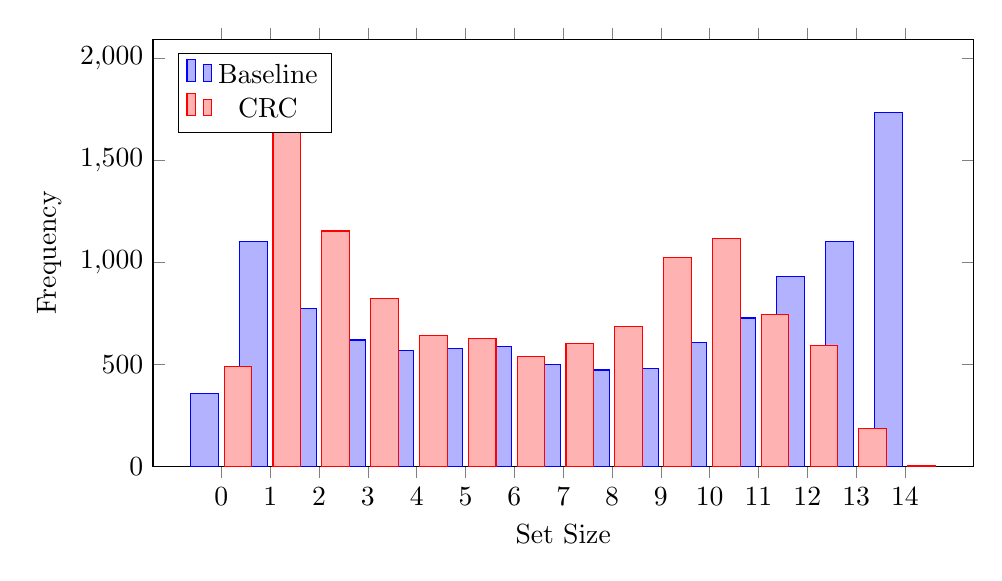
\begin{tikzpicture}
\begin{axis}[
    width=12cm,
    height=7cm,
    ybar,
    xtick=data,
    ylabel={Frequency},
    % xticklabel style={
    %     font=\footnotesize,
    %     rotate=45,
    %     anchor=east
    % },
    xlabel={Set Size},
    ymin=0,
    enlarge x limits=0.10,
    legend pos=north west,
]

\addplot coordinates {
    (0, 356)
    (1, 1101)
    (2, 773)
    (3, 619)
    (4, 567)
    (5, 578)
    (6, 588)
    (7, 499)
    (8, 472)
    (9, 478)
    (10, 605)
    (11, 727)
    (12, 929)
    (13, 1101)
    (14, 1735)
};
\addlegendentry{Baseline}

\addplot coordinates {
  (0, 488)
  (1, 1900)
  (2, 1153)
  (3, 824)
  (4, 641)
  (5, 625)
  (6, 539)
  (7, 602)
  (8, 686)
  (9, 1022)
  (10, 1115)
  (11, 746)
  (12, 594)
  (13, 187)
  (14, 6)
};
\addlegendentry{CRC}

\end{axis}
\end{tikzpicture}

\end{document}
